\chapter{Doelen \& Motivatie}
\label{hoofdstuk:doelen}

Het hoofddoel van het thera project is om het volledige proces van fresco's reconstrueren zo gemakkelijk mogelijk te maken. Er moet een manier gevonden worden om een waardevolle contributie te maken aan het thera-ecosysteem zodat het zijn doel beter kan vervullen. Dit is onder andere mogelijk door delen die ontbreken aan de vorige oplossingen aan te maken of bestaande componenten veelzijdiger te maken.\\

Gezien de huidige stand van zaken besproken in hoofstuk \ref{hoofdstuk:overzicht}, valt het op dat er nog behoorlijk wat dingen kunnen toegevoegd worden op het gebied van informatie en het visualiseren ervan. De ongelooflijke hoeveelheid data die het thera project reeds heeft geproduceerd en blijft produceren kan op een betere manier behandeld worden zodat het ware potentieel ervan naar de oppervlakte komt. De laatste stap in het sterk geautomatiseerde virtuele reconstructie proces wordt gekenmerkt door een nood aan interactie met de mens die elk soort hulpmiddel moet krijgen om een beslissing zo correct en snel mogelijk te maken. Natuurlijk gaat er niets boven de feitelijke fragmenten fysisch vastnemen en ze aan elkaar te proberen zetten. Maar gezien dit een zeer tijdsrovende bezigheid is, moet dit zo veel mogelijk beperkt worden.\\

Er werd gesproken over Griphos en diens weinig ontwikkelde ondersteuning voor het behandelen van automatisch voorgestelde fragmentparen, alsook over de eerste poging om dit recht te trekken: Browsematches. Deze thesis tracht de lijn van Browsematches verder te zetten, vertrekkende van de goede idee\"en en ervaring waaraan het zijn ontstaan te danken heeft. Dit houdt in dat de focus niet meer zozeer ligt op het actief puzzelen en brokstukken op een tafelblad plaatsen, maar eerder op het beoordelen van de omvangrijke verzameling voorstellen, waarvan slechts een zeer klein deel correct kan zijn. De hoop en verwachting is dat dit zeer kleine deel meteen ook een significante hoeveelheid van de werkelijk overblijvende paren voorstelt.\\

Daarmee valt te benadrukken dat dit project geen vervanging probeert te zijn van de bestaande software, het is eerder bedoeld als een complement. Merk op dat gevalideerde paren niet kunnen conflicteren en dus rechtstreeks in een groep op een tafelblad geplaatst kunnen worden. In de limiet, wanneer alle mogelijke paren correct geclassificeerd zijn vloeit hieruit op natuurlijk wijze een (zo compleet mogelijk) fresco voort. Daarom valt de implementatie in de thesis te zien als een extra tussenstap, chronologisch v\'o\'or het plaatsen van de fragmenten op een tafelblad en na het uitvoeren van de herkenningsalgoritmen. Figuur \ref{fig:flow} stelt dit visueel voor.

\begin{figure}[ht]
	\begin{center}
		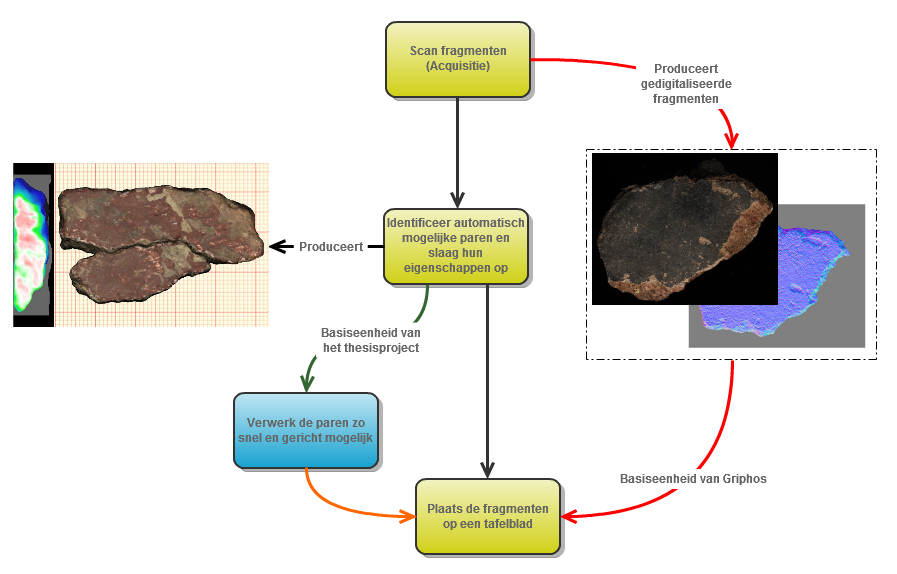
\includegraphics[width=1.0\columnwidth]{images/flowchart-focus-01.png}
		\caption{Het huidige proces met de aanvullingen van de thesis in het blauw}
		\label{fig:flow}
	\end{center}
\end{figure}

Een van de meest fundamentele verschillen tussen de centrale filosofie die Griphos vooropstelt en die van dit project is dus dat terwijl bij Griphos de focus ligt op aparte geplaatste fragmenten, het thesisproject eerder de automatische gevonden paren behandelt. Het is in Griphos wel degelijk mogelijk om voorstellen van de automatische paarherkenning in te laden maar de naald in de hooiberg vinden is moeilijk.\\

\section{Aspecten waarop de thesis tracht te verbeteren}
Hieronder beschreven staan verschillende deelaspecten waarop dit thesisproject tracht verbeteringen (op Browsematches) te maken. Bij elk aspect staat een beschrijving van wat het resultaat allemaal zou moeten mogelijk maken. Men kan deze desgewenst onafhankelijk bekijken maar vaak steunen ze op elkaar om werkelijk tot hun recht te komen. Wat is bijvoorbeeld een visualisatiemethode zonder een manier om de zaken die men wil zien te kiezen en aan te reiken? Wat is een uitgebreid databeheersysteem zonder een mogelijkheid om eigenlijk iets met deze data te doen? Om de verbeteringen en idee\"en te bundelen en te testen is er ook een applicatie gemaakt die dient om reeds een voorproef te geven van wat er mogelijk is met de ontwikkelde technologie.  

\subsection{Integratie}
Zoals eerder vermeld staat dit thesisproject niet alleen maar maakt het deel uit van een groter geheel. Binnen de grenzen van het mogelijke zou er moeten rekening gehouden worden met de integratie van de geschreven code met die van de andere onderzoekers. Dit verhoogt de kans dat het werk aanvaard wordt en ingang vindt in andere subprojecten. 

\subsection{Collaboratie}
Ideaal gezien zouden archeologen steeds toegang moeten krijgen tot hun project op eender welk moment vanop eender welke plaats. Dit kan een gedeelde collectie zijn die over het internet beschikbaar wordt gesteld, of een lokale kopie. Een mogelijk scenario hierbij is dat een ervaren archeoloog in de Verenigde Staten gevraagd wordt om zijn opinie te geven over de huidige stand van zaken (reeds ge\"identificeerde correcte paren, moeilijke gevallen, \ldots). Alle aanpassingen en commentaren die hij maakt worden automatisch ingevoegd en centraal beschikbaar gesteld voor de onderzoekers ter plekke. Op termijn moet het bijvoorbeeld zelfs mogelijk worden om amateurs te laten kijken naar de voorstellen en hun beoordeling te gebruiken om de nog na te kijken voorstellen te rangschikken.

Van cruciaal belang is dat alle verzamelde data (zoals de classificatie van voorstellen) op een robuuste manier opgeslagen, gedeeld en ge\"incorporeerd kan worden. De toegang naar en manipulatie van deze informatie moet effici\"ent zijn. De huidige oplossingen zijn hiervoor ontoereikend en traag, zoals besproken in hoofdstuk \ref{hoofdstuk:overzicht}. De mogelijkheid van meerdere en zelfs lokale kopie\"en impliceert ook de nood om te kunnen synchroniseren\footnote{Naar het model van de zogenaamde \emph{Distributed Version Control System (DCVS)} systemen zoals Git, Mercurial, \ldots}. Dit is ook nodig omdat er reeds verschillende huidige verzamelingen bestaan die eventueel in het nieuwe systeem ge\"importeerd en gecombineerd moeten worden. Dergelijk systeem is ook nuttig voor het maken van (kleinere) pocketversies en in gebieden waar de internetconnectiviteit niet adequaat of onbestaande is. Belangrijk is dat er steeds een manier is om waardevolle data te combineren en aan te vullen zodat niets verloren gaat.\\

\subsection{Schalering}
De bestaande oplossingen voor het valideren van voorgestelde paren werken noodgedwongen met een sterk gereduceerde verzameling. E\'en van de redenen hiervoor is het gebruik van een groot XML bestand om alles in op te slaan. Deze techniek werkt goed voor bijvoorbeeld het opslaan van tafelbladen --- waar er bijvoorbeeld 50 fragmenten en hun locaties moeten opgeslagen worden --- maar schiet tekort voor paarvoorstellen. Een snelle rekensom geeft de reden aan: een laag aantal fragmenten voor een specifieke opgraving is bijvoorbeeld 1500. De meeste paarherkenners gaan alle brokstukken een keer met elk andere brokstuk vergelijken en zodoende het meest waarschijnlijke aankoppelingspunt vinden. Het is zelfs mogelijk dat een fragment meerdere keren een plausibel paar vormt met eenzelfde stuk. Naar onder afgerond komen uit deze stap reeds 2 miljoen configuraties gerold, de ene wat waarschijnlijker dan de andere. Dit nummer stijgt kwadratisch in het aantal fragmenten en zelfs met hogere drempels om volgens een bepaalde maatstaf paren automatisch te verwerpen stijgt het aantal configuraties snel.

\subsection{Gebruiksvriendelijkheid}
De uiteindelijke gebruikers van de applicatie zijn niet de ontwikkelaars van het thera project zelf, maar de archeologen. Om deze reden is het belangrijk dat er rekening gehouden wordt met de noodzaak van een visueel aangename en intuiti\"eve gebruikservaring. Om deze intu\"itiviteit te bereiken moet in het programma steeds de aandacht gevestigd blijven op hetgeen het belangrijkst en meest herkenbaar is: de paren en hun fragmenten. Bij voorkeur moet elke operatie gemakkelijk ontdekbaar zijn in de context waar ze kan gebruikt worden, met eventueel een woordje uitleg erbij.\\

Volgens vele studies op het gebied van gebruikersinterfaces \cite{Hoxmeier00,Shneiderman84,Nielsen94} geraken gebruikers gefrustreerd vanaf een operatie een zekere tijd duurt. Deze frustratiedrempel hangt een af van de aard van de operatie (het resultaat), de frequentie waarmee die uitgevoerd wordt, of er visuele tekenen van voortgang zijn en of er tijdens het wachten (steeds) iets anders kan uitgevoerd worden. Om deze reden is het belangrijk dit aspect in acht te nemen bij het ontwikkelen van de applicatie. Dit is vooral zo omdat veel van de acties die mogelijk moeten zijn het potentieel hebben traag te lopen en dus de gebruiker te frustreren. Een algemene vaststelling: de tijd die een operatie mag innemen is omgekeerd evenredig met de frequentie waarmee deze operatie moet uitgevoerd worden. Deze regel in acht nemend is het duidelijk dat bijvoorbeeld het inladen van een scherm vol voorstellen zoals bij Browsematches, het veranderen van een attribuut van een paar, het filteren en sorteren en dergelijke meer acties zijn die met de grootst mogelijke snelheid moeten worden uitgevoerd. Hoe functioneel ook, een programma dat sloom reageert en elke computer op z'n knie\"en dwingt zal zo weinig mogelijk gebruikt worden \cite{Joel2001}.\\

// hoort mss bij [DESIGN]
De gebruikersinterface van de oude programma's was goed en kon effici\"ent gebruikt worden mits enige training. Maar voor het ondersteunen van collaboratief werken moeten er natuurlijk allerhande nieuwe operaties toegevoegd
worden. Tijdens het implementatieproces werd het duidelijk dat de reeds bestaande code van het Browsematches niet uitbreidbaar genoeg was en die van Griphos te complex en belangrijk. Daardoor werd de beslissing genomen om de
basisinterface van Browsematches over te nemen maar alle onderliggende code te herschrijven zodat die uitbreidbaar zou zijn. Bij het opnieuw construeren van dit alles zijn er een aantal verbeteringen gebeurd die niet meteen te maken hebben met het collaboratie aspect maar wel met de workflow van het classificeren. Dit werd gedaan om het hele programma gebruiksvriendelijker en krachtiger te maken in functie van het hoofddoel van het project.

\subsection{Uitbreidbaarheid}
Het samenstellen van werken uit de oudheid is een zeer vakkennis- en ervaringsintensief proces. Hoewel men luistert naar wat de archeologen hierover te vertellen hebben --- wat ze graag zouden zien of kunnen doen --- zijn er vele zaken die nu nog niet duidelijk zijn maar in de toekomst zeker aan het licht zullen komen. Dit kan bijvoorbeeld zijn omdat de onderzoekers in kwestie niet goed kunnen uitleggen waar ze naar kijken of hoe ze zoeken: na zovele jaren vertrouwen ze op hun moeilijk te defini\"eren intu\"itie. Anderzijds is het vertalen van het proces om fresco's samen te stellen naar de computer nog niet zo vaak geprobeert in het verleden. Dit betekent dat een goede werkwijze in de realiteit misschien niet zonder meer de effici\"entste is als men de transitie naar virtueel reconstrueren maakt (zoals bij Griphos). Daarbovenop zijn er nog vele kansen om innovatieve nieuwe technieken aan te wenden die niet werkbaar zijn als men enkel over fysische fragmenten beschikt.\\

Het is dus onwaarschijnlijk dat het laatste woord over de ideale metafoor reeds gezegd is waardoor er een grote kans is dat het platform zal moeten vervangen of herbouwd worden als het niet met uitbreidbaarheid in gedachte ontworpen wordt. Er moeten moeiteloos nieuwe delen aan de applicatie en de onderliggende lagen kunnen toegevoegd worden om snel nieuwe idee\"en te incorporeren. Dit alles moet best mogelijk zijn zonder de ervaring van gebruikers met oudere versies of andere gebruikersinterfaces te degraderen.

\subsubsection{Data}
De eerder besproken uitbreidbaarheid die nodig is manifesteert zich op het niveau van de data bijvoorbeeld bijboorbeeld op deze manier: een onderzoeker vindt een nieuw algoritme om fragmentparen te rangschikken op ``goedheid'' of men wil informatie over het dikteverschil tussen twee fragmenten opslaan. Idealiter zouden deze zaken als een attribuut bij een paar moeten kunnen toegevoegd worden zodat elke gebruiker er op kan zoeken en sorteren zonder iets extra te hoeven doen.\\
 
Enkel data die op geen enkele manier om te vormen valt naar een attribuut van een enkel paar zal een speciale module vereisen om te kunnen gebruiken. Een vereiste is natuurlijk wel dat dit geen effect mag hebben op de delen van het platform die hier geen weet van hebben.
 
\subsubsection{Visualisatie}
Er zijn vele visualisatiemanieren denkbaar die elkaar kunnen aanvullen bij het volbrengen van het zoek- en classificeerprocess. Zo stelt men zich bij de uitdrukking ``fresco's samenstellen'' waarschijnlijk een grote puzzel voor waar men ten alle tijde het overzicht kan behouden en stukken proberen te passen.\footnote{Het Griphos programma gaat uit van het idee van kleine beheersbare stukken van de reuzenpuzzel (elk tafelblad zou een verzameling kunnen zijn van stukken die gerelateerd waren, bijvoorbeeld door hun vindplaats)} Deze puzzel visualisatie is visueel aantrekkelijk en biedt het menselijke patroonherkenningsvermogen\footnote{Iets waar computers de mens nog altijd niet in evenaren. Een ander thera subproject onderzoekt wel de mogelijkheid om zogenaamde 'clusters' te identificeren en te gebruiken voor reconstructie.} de mogelijkheid om zich van zijn beste kant te laten zien. Echter, door de grote hoeveelheid aan fragmenten en dus mogelijke paren is het moeilijk om hier aan te beginnnen. Maar, hoe meer reeds geconfirmeerde paren er zijn, hoe duidelijker het globale beeld kan worden. Dit staat toe om een overzicht te krijgen van de vooruitgang en gerichter te zoeken naar stukken die nog ontbreken. Dit is een voorbeeld van een macro-perspectief.\\

Een alternatief is te beginnen door te kijken naar waar de computer w\'el goed in is: fragmenten aan elkaar passen en rangschikken naar kans/overeenkomst/et cetera. Door een gemakkelijk navigeerbare lijst op te stellen van alle voorstellen die de reconstructie algoritmes hebben gedaan, kunnen er snel op elkaar passende fragmenten ge\"identificeerd worden. Dit kan men zien als een micro-perspectief of \emph{bottom-up} manier om fresco's te reconstrueren. Het is ook de aanpak die in Browsematches gebruikt wordt. Nadat men bijvoorbeeld met deze manier een deel acceptabele paren heeft ge\'identificeerd, kunnen deze bijvoorbeeld weergegeven worder als een grote puzzel en dienen zij als beginpunt om verder te puzzelen. Dit maakt het globale beeld veel informatiever: stel dat duidelijke "gaten" ontstaan in een resem goede fragmentparen, dan kan er gericht gezocht worden naar een fragment dat erin past door te zoeken naar een fragment dat met elk van deze insluiters past (indien het gevonden werd bij de opgraving).\\

Kortom, het is duidelijk dat een visualisatie die in alle gevallen de meest geschikte is niet bestaat. De beschikbare informatie moet soms gewoon op andere manieren worden weergegeven. Om deze reden is het wenselijk om het mogelijk te maken snel nieuwe visualisaties in te bouwen die kunnen communiceren met andere delen van de applicatie en eventueel de informatie manipuleren. 